\documentclass[twocolumn]{article}
\usepackage[utf8]{inputenc}
\usepackage{amsfonts,amsmath,amssymb}
\usepackage[brazil]{babel}
\usepackage{lipsum}
\usepackage{graphicx}


% Isto é um comentário.
\author{Nome do mecânico} %autor
\date{\today} %data
\title{Oficina de \LaTeX} %título


\begin{document}
\maketitle % % % Produz a capa

\begin{abstract}
Este documento visa fornecer noções básicas sobre o sistema de formatação de texto \LaTeX.
\end{abstract}
\section{Introdução}
\lipsum[3]
\section{Tópicos}
Para dispor as informações em tópicos, utilizamos o ambiente {\tt itemize}:
\begin{itemize}
	\item Primeiro item.
	\item Segundo item.
	\item Terceiro item.
\end{itemize}

\subsection{Enumerações}

Também é possível fazer enumerações em forma de tópico, basta utilizar o ambiente {\tt enumerate}.
\begin{enumerate}
	\item Um, dois, feijão com arroz.
	\item três, quatro, feijão no prato.
	\item cinco, seis, pão francês.
\end{enumerate}

\section{Modo Matemático}
Vamos ilustras algumas coisas que podemos fazer no modo matemático:
\begin{itemize}
\item Fórmula de Bhaskara:

\begin{equation}
	a^2 = b^2 + c^2
	\label{eq:bhaskara}
\end{equation}
De acordo com a Equação \ref{eq:bhaskara}, o quadrado da hipotenusa é igual a soma dos quadrados dos catetos.

\item Integrais: a Integral \ref{eq:integral} corresponde à integral definida de $f(x)$ no intervalo $[a,b]$.
\begin{equation}
\int_{a}^{b} f(x)\,d(x)
\label{eq:integral}
\end{equation}

\item Relação de recorrência:
\begin{equation}
M(i,j) = \max \left\{
\begin{array}{l}
M(i,j-1)\\
M(i-1,j-1)+\delta(i,j)\\
M(i-1,j)
\end{array} \right.
\label{eq:recorrencia}
\end{equation}

A Equação \ref{eq:recorrencia} corresponde à relação de recorrência do problema da maior subsequência comum ($\mathcal{LCS}$).

\end{itemize}




\section{Figuras}

Para colocar figuras, utilizamos o ambiente {\tt figure}:

\begin{figure}[h!]
\centering
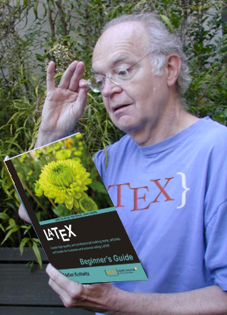
\includegraphics[scale=.7]{figuras/Knuth}
\caption{Donald Knuth, o criador do \TeX.}
\label{fig:Knuth}
\end{figure}



\begin{figure}[h!]
\centering
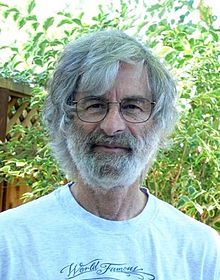
\includegraphics[scale=.7]{figuras/Lamport}
\caption{Leslie Lamport, o criador do \LaTeX.}
\label{fig:Lamport}
\end{figure}



Nas Figuras \ref{fig:Knuth} e \ref{fig:Lamport}, podemos ver respectivamente Donald Knuth e Leslie Lamport.


\section{Tabelas}

\begin{table}[h!]
\centering
\caption{Dígitos de um Telefone}
\begin{tabular}{|c|c|c|}
\hline
1 & 2 & 3\\\hline
4 & 5 & 6\\\hline
7 & 8 & 9\\\hline
* & 0 & \#\\\hline
\end{tabular}
\label{tab:matriz}
\end{table}


\begin{figure}[h!]
\centering

\includegraphics[scale=.6]{figuras/this-is-dog}
\caption{Hello, this is dog!}
\label{fig:cachorro}
\end{figure}

Os dígitos do telefone, ilustrados pela Tabela \ref{tab:matriz}, foram utilizados pelo cachorro da Figura
\ref{fig:cachorro}.

\section{Referenciando Objetos}
Como disposto neste documento, para referenciar objetos, basta utilizar o comando {\tt $\backslash$ref}.
\section{Citações}
Para usar citações, utilizamos o comando {$\backslash$cite}.

Leslie Lamport, ilustrado pela Figura, teve uma importância muito grande, ao escrever uma sequência de comandos para o \TeX, que possibilitava o seu uso em mais alto nível.

O \TeX por sua vez, foi desenvolvido por Donald Knuth, ilustrado pela Figura,  durante a escrita da sua obra clássica, The Art of Computer Programming \cite{Knuth81}.

Ambos autores, publicaram trabalhos sobre o \TeX{} e o \LaTeX, conforme visto em \cite{knuth1979tex} e \cite{lamport1986document}.

\section{Conclusão}
Concluímos que o \LaTeX é um sistema tipográfico extremamente importante nas mais diversas áreas, visto que proporciona uma qualidade tipográfica sem igual e um grande suporte a textos matemáticos, referências a objetos e citações.
\subsection{Agradecimentos}
Agradeço a todos os participantes da SECITEC por comparecerem à oficina. Espero que tenham aprendido algo de \LaTeX.

\bibliographystyle{amsalpha}
\bibliography{bibliografia}

\end{document}}